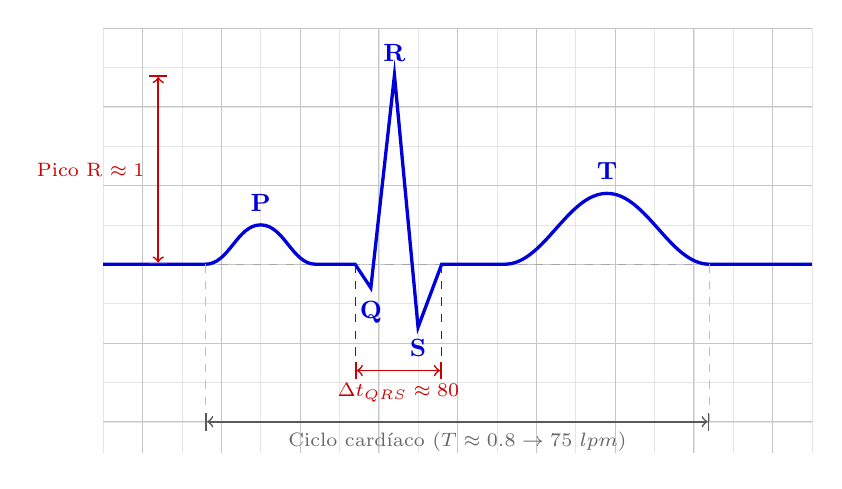
\begin{tikzpicture}[transform shape]
  % Cuadricula en tonos grises acorde a las graficas tecnicas del informe
  \draw[step=0.5, color=gray!20, line width=0.1pt] (-0.5, -2.4) grid (8.5, 3.0);
  \draw[step=1.0, color=gray!45, line width=0.25pt] (-0.5, -2.4) grid (8.5, 3.0);

  % Linea isoelectrica de referencia (0 V)
  \draw[dashed, color=gray!70, line width=0.5pt] (-0.5, 0) -- (8.5, 0);

  % Trazado de la senal de biopotencial ECG en azul (curva principal)
  \draw[color=blue!85!black, very thick, smooth] 
    (-0.5, 0) -- (0.8, 0) 
    .. controls (1.1, 0) and (1.2, 0.5) .. (1.5, 0.5)
    .. controls (1.8, 0.5) and (1.9, 0) .. (2.2, 0)
    -- (2.7, 0)
    -- (2.9, -0.3) % Q
    -- (3.2, 2.4)  % R
    -- (3.5, -0.8) % S
    -- (3.8, 0)    % Punto J
    -- (4.6, 0)
    .. controls (5.1, 0) and (5.4, 0.9) .. (5.9, 0.9)
    .. controls (6.4, 0.9) and (6.7, 0) .. (7.2, 0)
    -- (8.5, 0);

  % Identificacion clara de las ondas P, Q, R, S, T
  \node[above, font=\bfseries\small, color=blue!85!black] at (1.5, 0.55) {P};
  \node[below, font=\bfseries\small, color=blue!85!black] at (2.9, -0.35) {Q};
  \node[above, font=\bfseries\small, color=blue!85!black] at (3.2, 2.45) {R};
  \node[below=1pt, font=\bfseries\small, color=blue!85!black] at (3.5, -0.8) {S};
  \node[above, font=\bfseries\small, color=blue!85!black] at (5.9, 0.95) {T};

  % Cota vertical de amplitud de pico R (en rojo sutil)
  \draw[|<->|, semithick, color=red!80!black] (0.2, 0) -- (0.2, 2.4);
  \node[anchor=east, font=\scriptsize, color=red!80!black] at (0.15, 1.2) {Pico R $\approx \SI{1}{\milli\volt}$};

  % Cota de duracion temporal del complejo QRS (determina frecuencia de corte fH)
  \draw[dashed, color=red!60!black, line width=0.35pt] (2.7, 0) -- (2.7, -1.35);
  \draw[dashed, color=red!60!black, line width=0.35pt] (3.8, 0) -- (3.8, -1.35);
  \draw[|<->|, semithick, color=red!80!black] (2.7, -1.35) -- (3.8, -1.35);
  \node[below=1pt, font=\scriptsize\bfseries, color=red!80!black] at (3.25, -1.35) {$\Delta t_{\text{QRS}} \approx \SI{80}{\milli\second}$};

  % Cota del ciclo cardiaco completo (determina frecuencia fundamental f0)
  \draw[dashed, color=gray!50, line width=0.35pt] (0.8, 0) -- (0.8, -2.0);
  \draw[dashed, color=gray!50, line width=0.35pt] (7.2, 0) -- (7.2, -2.0);
  \draw[|<->|, semithick, color=gray!70!black] (0.8, -2.0) -- (7.2, -2.0)
    node[midway, below, font=\scriptsize, color=gray!80!black] {Ciclo cardíaco ($T \approx \SI{0.8}{\second} \rightarrow 75\ \text{lpm}$)};

\end{tikzpicture}
